\documentclass{article}
\usepackage{amsthm}
\usepackage{amssymb}
\usepackage{pgf, tikz}
\usetikzlibrary{arrows, automata}
\begin{document}
\title{Homework 11}
\author{Will Boland}
\maketitle

\textbf{Question 1}\newline
A) Function\newline

\textit{Proof}\newline
\textbf{First Requirement}\newline
Choose x $\in$ $\mathbb{R}$.\newline
 Let y = 3x-5\newline
3, 5, and x are real numbers, so therefore y is a real number\newline
y + 5 = 3x - 5 + 5\newline
= 3x\newline
That means L(x, y)\newline
\textbf{Second Requirement}\newline
Choose real numbers x, y, and z and assume that L(x, y) and L(x, z)\newline
so we know y + 5 = 3x and z + 5 = 3x\newline
y + 5 = z + 5\newline
y = z $\square$\newline\newline

B) Partial, but not total function\newline
Counter example for first requirement: (0, 2) $\notin$ P1 but 0 $\in$ $\mathbb{Z}$ and 2 $\in$ $\mathbb{Z}$\newline

\textit{Proof}\newline
\textbf{Second Requirement}\newline
Choose numbers x, y, and z and assume P1(x, y) and p1(x, z)\newline
So we know x * y = 6 and x * z = 6\newline
So x = 6/y and x = 6/z\newline
6/y = 6/z$\square$\newline\newline

C) Partial, but not total function\newline
Counter example for first requirement: (0, 2) $\notin$ P1 but 0 $\in$ $\mathbb{Z}$ and 2 $\in$ $\mathbb{Z}$\newline

\textit{Proof}\newline
\textbf{Second Requirement}\newline
Choose numbers x, y, and z and assume P1(x, y) and p1(x, z)\newline
So we know x * y = 6 and x * z = 6\newline
So x = 6/y and x = 6/z\newline
6/y = 6/z$\square$\newline\newline

D) Not a function because S("xbox", "hell")  and S("xbox", "many") so one input has two outputs therefore not a function\newline\newline


\textbf{Question 2}\newline
A) \{(a, b), (b, a), (c, b)\}\newline
B) Psee graph \newline
\begin{tikzpicture}[
            > = stealth, % arrow head style
            shorten > = 1pt, % don't touch arrow head to node
            auto,
            node distance = 3cm, % distance between nodes
            semithick % line style
        ]

        \tikzstyle{every state}=[
            draw = black,
            thick,
            fill = white,
            minimum size = 4mm
        ]

	\node[state] (a) {$a$};
	\node[state] (b) [right of=a] {$b$};
	\node[state] (c) [right of=b] {$c$};
	\node[state] (1) [below of=a] {$1$};
	\node[state] (2) [below of=b] {$2$};
	\node[state] (3) [below of=c] {$3$};
	\node[state] (4) [right of=3] {$4$};
	
        \path[->] (a) edge node {} (1);
        \path[->] (b) edge node {} (2);
        \path[->] (c) edge node {} (3);

    \end{tikzpicture}
\newline\newline
C) see graph\newline
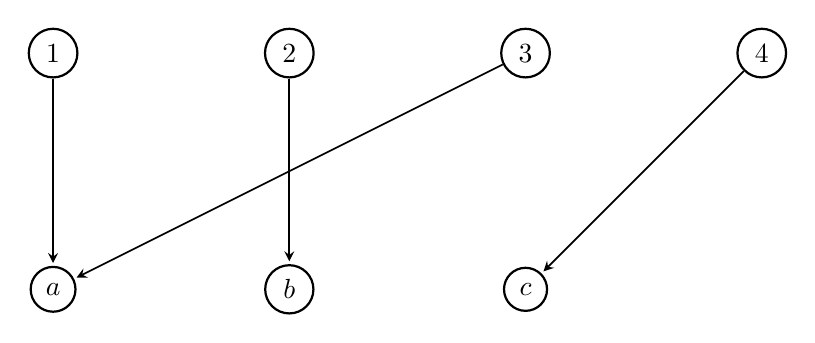
\begin{tikzpicture}[
            > = stealth, % arrow head style
            shorten > = 1pt, % don't touch arrow head to node
            auto,
            node distance = 3cm, % distance between nodes
            semithick % line style
        ]

        \tikzstyle{every state}=[
            draw = black,
            thick,
            fill = white,
            minimum size = 4mm
        ]

	\node[state] (1) {$1$};
	\node[state] (2) [right of=1] {$2$};
	\node[state] (3) [right of=2] {$3$};
	\node[state] (4) [right of=3] {$4$};
	\node[state] (a) [below of=1] {$a$};
	\node[state] (b) [below of=2] {$b$};
	\node[state] (c) [below of=3] {$c$};
	
	\path[->] (1) edge node {} (a);
	\path[->] (2) edge node {} (b);
	\path[->] (3) edge node {} (a);
	\path[->] (4) edge node {} (c);

    \end{tikzpicture}
\newline\newline
D) f(x) = ${x^2}$\newline
E) f(x) = $\mid$${x^2}$$\mid$\newline
F) f = \{(x, y) $\mid$ y = number of true assignments in x\newline\newline


\textbf{Question 3}\newline
A) f(x) = x\newline
B) Impossible because if it is not onto, we will not use at least one of our codomains; however, for it to be one-to-one we would need one output to have only one input corresponding to it; therefore making it impossible.\newline
C) Impossible because in in order for the function to NOT be one-to-one, then there must exist an output that has two inputs; however, to be onto, each output (codomain) must have at least one input to map to it. Yet, no input can have two outputs\newline
D) see graph\newline
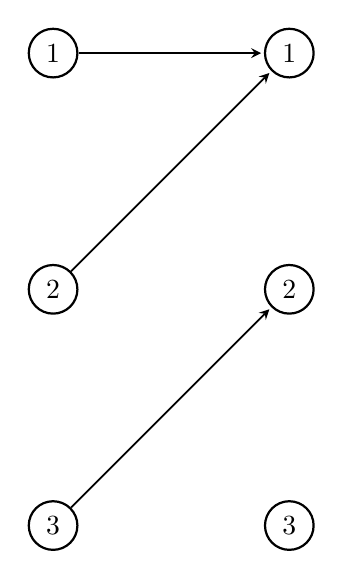
\begin{tikzpicture}[
            > = stealth, % arrow head style
            shorten > = 1pt, % don't touch arrow head to node
            auto,
            node distance = 3cm, % distance between nodes
            semithick % line style
        ]

        \tikzstyle{every state}=[
            draw = black,
            thick,
            fill = white,
            minimum size = 4mm
        ]

	\node[state] (1) {$1$};
	\node[state] (2) [below of=1] {$2$};
	\node[state] (3) [below of=2] {$3$};
	\node[state] (11) [right of=1] {$1$};
	\node[state] (22) [below of=11] {$2$};
	\node[state] (33) [below of=22] {$3$};
	
	\path[->] (1) edge node {} (11);
	\path[->] (2) edge node {} (11);
	\path[->] (3) edge node {} (22);

    \end{tikzpicture}
\newline\newline
E) f(x) = the letter at index x where the index starts at 1 instead of the usual 0\newline
F) Impossible because there are 3 members of the domain but 4 members of the codomain, meaning that inorder for the domain to be onto, one input would have to have more than one output; therefore, it could not be a function\newline
G) see graph\newline
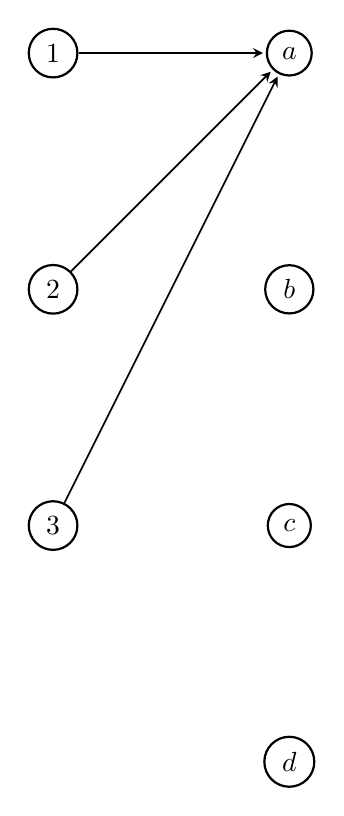
\begin{tikzpicture}[
            > = stealth, % arrow head style
            shorten > = 1pt, % don't touch arrow head to node
            auto,
            node distance = 3cm, % distance between nodes
            semithick % line style
        ]

        \tikzstyle{every state}=[
            draw = black,
            thick,
            fill = white,
            minimum size = 4mm
        ]

	\node[state] (1) {$1$};
	\node[state] (2) [below of=1] {$2$};
	\node[state] (3) [below of=2] {$3$};
	\node[state] (a) [right of=1] {$a$};
	\node[state] (b) [below of=a] {$b$};
	\node[state] (c) [below of=b] {$c$};
	\node[state] (d) [below of=c] {$d$};
	
	\path[->] (1) edge node {} (a);
	\path[->] (2) edge node {} (a);
	\path[->] (3) edge node {} (a);

    \end{tikzpicture}
\newline\newline
H) impossible because our domain has 4 inputs but our codomain has 3 outputs, so therefore at least one input will share an output with another input\newline
I) see graph\newline
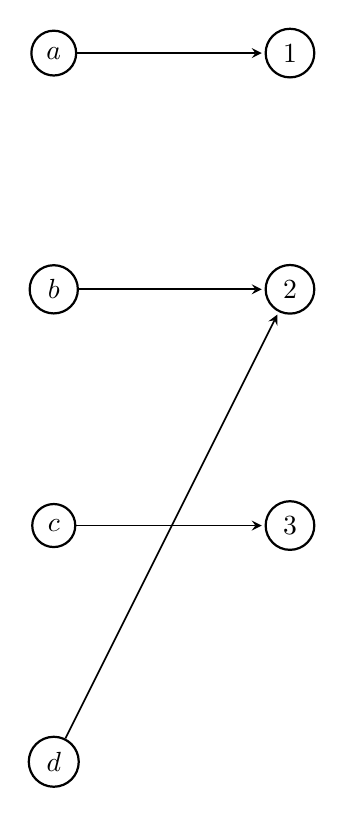
\begin{tikzpicture}[
            > = stealth, % arrow head style
            shorten > = 1pt, % don't touch arrow head to node
            auto,
            node distance = 3cm, % distance between nodes
            semithick % line style
        ]

        \tikzstyle{every state}=[
            draw = black,
            thick,
            fill = white,
            minimum size = 4mm
        ]

	\node[state] (a) {$a$};
	\node[state] (b) [below of=a] {$b$};
	\node[state] (c) [below of=b] {$c$};
	\node[state] (d) [below of=c] {$d$};
	\node[state] (1) [right of=a]{$1$};
	\node[state] (2) [below of=1] {$2$};
	\node[state] (3) [below of=2] {$3$};
	
	\path[->] (a) edge node {} (1);
	\path[->] (b) edge node {} (2);
	\path[->] (c) edge node {} (3);
	\path[->] (d) edge node {} (2);


    \end{tikzpicture}
\newline\newline
J) see graph\newline
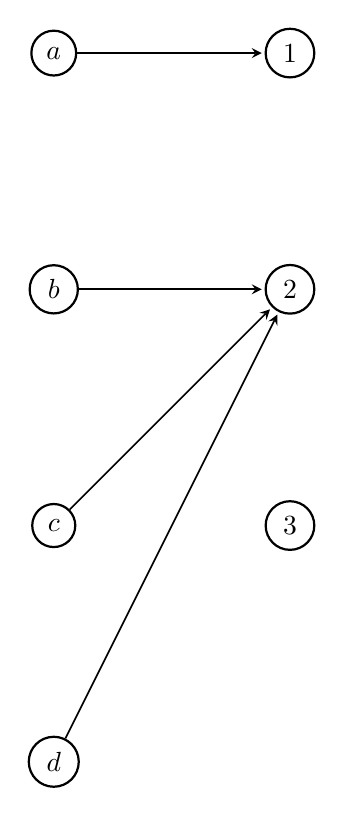
\begin{tikzpicture}[
            > = stealth, % arrow head style
            shorten > = 1pt, % don't touch arrow head to node
            auto,
            node distance = 3cm, % distance between nodes
            semithick % line style
        ]

        \tikzstyle{every state}=[
            draw = black,
            thick,
            fill = white,
            minimum size = 4mm
        ]

	\node[state] (a) {$a$};
	\node[state] (b) [below of=a] {$b$};
	\node[state] (c) [below of=b] {$c$};
	\node[state] (d) [below of=c] {$d$};
	\node[state] (1) [right of=a]{$1$};
	\node[state] (2) [below of=1] {$2$};
	\node[state] (3) [below of=2] {$3$};
	
	\path[->] (a) edge node {} (1);
	\path[->] (b) edge node {} (2);
	\path[->] (c) edge node {} (2);
	\path[->] (d) edge node {} (2);


    \end{tikzpicture}
\newline\newline
K) f(x) = x + 1\newline
L) f(x) = $x^4$\newline
M) f(x) = ${x^3}$ - 9x\newline
N) f = \{(x, y) $\mid$ y = x mod 2\}\newline\newline

\textbf{Question 4}\newline
A) \textit{Proof}\newline
Choose ${x_1}$, ${x_2}$ $\in$ $\mathbb{R}$ and assume f(${x_1}$) = f(${x_2}$)\newline
So 2${x_1}$ - 7 = 2${x_2}$ - 7\newline
2${x_1}$ = 2${x_2}$\newline
${x_1}$ = ${x_2}$$\square$\newline\newline
B) \textit{Proof}\newline
Choose y $\in$ $\mathbb{R}$\newline
Let x = (y + 7) / 2\newline
Since y, 2, and 7 are real numbers, so is x\newline
x = (y + 7) / 2\newline
2x = y + 7\newline
2x - 7 = y$\square$\newline\newline

\textbf{Question 5}\newline
A) g(6) = 9 and g(0) = 9 so therefore not one-to-one\newline
B) g(-2) = 25, which is equal to ${(-2 - 3)^2}$ and any number squared is positive therefore any x where x - 3 < 0 will be positive\newline\newline

\textbf{Question 6}\newline
A) h("A-B-C-D") = "ABCD" AND H("A-B---C------D") = "ABCD"\newline
B) h("---------") \newline\newline

\textbf{Question 7}\newline
A) m(\{3, 4, 5, 6, 7\}) = 3 and m(\{3, 6, 10, 2000000\}) = 3

\enddocument
